Our dataset contains $3414$ object segmentations from the Pascal-S dataset. For this analysis, we first assigned three in-house annotators the task of assigning class labels to each object segmentation in our dataset. The annotators were given the original image (for reference) and the object segmentation and asked to assign $1$ category to the segment out of $7$ possible categories: animal, building, device, furniture, nature, person, and vehicle. We choose these high-level categories such that a wide range of object classes could be covered under these categories. For example, device included object segments like utensils, bottle, tv, computer etc, nature included segments like tree, mountain, flowers, and vehicle covered segments like car, bike, bus, aeroplane etc. \textcolor{red}{add a small table here which shows stats of the object classes n their frequency in the dataset.}

Figure \ref{fig:avgMem} shows the average memorability score for the all $7$ different object classes in our dataset. This visualisation gives a sense of how the memorability of different object classes differs. Animal, person, and vehicle are all highly memorable classes with each of them having an average memorability score greater than $0.5$. Interestingly, all the other object categories have an average memorability score lower than $0.25$ indicating that humans do not remember objects from these categories very well. In particular, furniture has an average memorability score of only $0.18$ and is the least memorable object class. This could be possibly due to the fact that most objects from classes like furniture, nature, and building either appear mostly in the background or are occluded which could decrease their memorability significantly. On the contrary, objects from animal, person, and vehicle classes appear mostly in the foreground leading to a higher memorability score on average. Table \ref{tab:avgMem} shows the average memorability of the top $20$ most memorable objects for each object class. This analysis is particularly interesting as these top objects are not occluded and most of them tend to appear in the foreground. The top $20$ most memorable objects from person, animal and vehicle have memorability higher than $0.90$ whereas the average memorability of the top $20$ objects from building, furniture, and nature is lesser than $0.70$. While the differences in the memorability of different classes could be driven primarily due to factors like occlusion, size, background/foreground, the results in table \ref{tab:avgMem} suggest that memorability could be an intrinsic property of an object class and some object classes like person, animal, vehicle are in general intrinsically more memorable than classes like furniture, nature etc.

\begin{table}
\begin{center}
    \begin{tabular}{| l | l |}
    \hline
    Object Class & Memorability of top $20$ objects \\ \hline
    Animal & 0.94  \\ \hline
    Building & 0.65  \\ \hline
    Device & 0.86  \\ \hline
    Furniture & 0.63  \\ \hline
    Nature & 0.67  \\ \hline
    Person & 0.93  \\ \hline
    Vehicle & 0.96  \\ \hline
    \end{tabular}
\end{center}
\caption {Average memorability of top $20$ objects for each class} \label{tab:avgMem}
\end{table}


\begin{figure}[t]
\centering
\subfigure{\centering 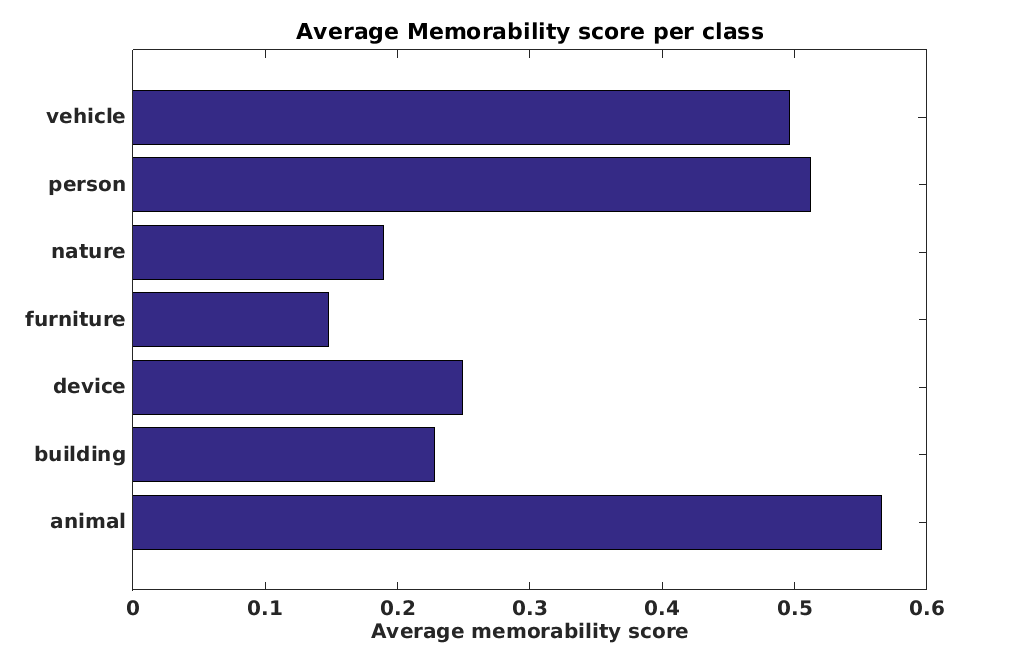
\includegraphics[width=0.4\textwidth]{figures/results/obLabel/Average_MemScore.png}}
\vspace{-5mm}\caption{\footnotesize\textbf{Average memorability per object class.} Figure showing some object classes are more memorable than others. }\label{fig:avgMem}
\end{figure} 